

\documentclass[float=false, crop=false]{standalone}
\usepackage[subpreambles=true]{standalone}
\usepackage{import}
\begin{document}
\chapter{Administration}
This is a whole chapter about administrative things for the supervisor. None of it is what the board writes, as they make changes at will. For example, \textcolor{orange}{Fourier series}
\marginnote{Fourier Series}
\index{Fourier series}
 gets indexed for no apparent reason.

Say, do you remember that image of space from last chapter? Here is the image, presented as a figure. Look how pretty a figure can be!
\begin{figure}[h]
    \centering
    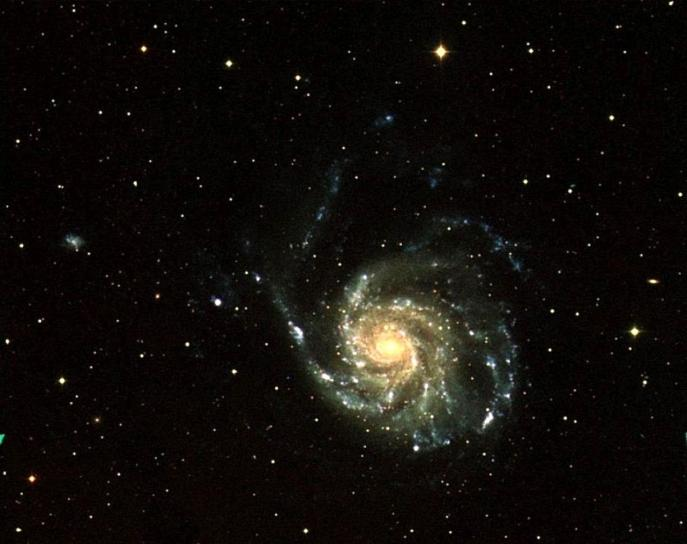
\includegraphics[width=0.25\textwidth]{space}
    \caption{a nice plot}
    \label{fig:space1}
\end{figure}
 
As you can see in the figure \ref{fig:space1}, the 
function grows near 0. Also, in the page \pageref{fig:space1} 
is the same example.
 
All of this continues to another page, which includes a bulleted list.
\begin{itemize}
\item fun
\item sun 
\item rock
\item roll
\item magic
\item fun
\item space
\item more
\item okay
\end{itemize}


The most important consideration is the use of power when microwaving burritos. Whether at a concert or anywhere that sells gasoline, burritos and microwaves are your friends. These are the friends you want to keep. Parents encourage their kids to have these lasting relationships. 

A \textcolor{orange}{TikZ}
\marginnote{TiKZ} 
\index{TikZ}
 figure will be rendered below this line. It has to get to the next page first. Be sure to hold your excitement for the moment. It really will be ready to show momentarily. Any old moment. Could be this one. Maybe now? 
 \begin{figure}[ht]
 \subimport{../}{diagram.tex}
 \label{fig:tikzexample}
\caption{A nice simple diagram}
\end{figure}
 ...
\end{document}


